\documentclass[12pt,a4paper]{article}
\usepackage[utf8]{inputenc}
\usepackage{amsthm}
\usepackage{amsmath}
\usepackage{amsfonts}
\usepackage{amssymb}
\usepackage{tikz}
\usetikzlibrary{trees}
\usepackage{bbold}
\usepackage{verbatim}
\usepackage{amsopn}
\usepackage{tikz}
\usepackage{algorithm}
\usepackage[noend]{algpseudocode}
\usepackage{MnSymbol}
\usepackage{subcaption}
\usetikzlibrary{arrows}
\usetikzlibrary{patterns}
\newtheorem{theorem}{Theorem}
\newtheorem{definition}{Definition}

\begin{document}
\title{Supervised Learning}
\maketitle

In a supervised learning problem we have a learning set $\mathcal S$ of 
$N$ observations, $\mathcal S = \{(x_i, y_i)\}_{i=1}^N$. Where $y_i$ are realizations of the so called target $Y$, which is a random variable (RV) with sample space (i.e., the space of all possible outcomes) $\Omega_t,  ~ \Omega_t \subseteq \mathbb R$. The $x_i$ are called feature vectors. They are realizations of a $p$-dimensional RV  $X=(X_1, \dots, X_p)^T$ with sampel space $\Omega$ and associated sample spaces of the scalar RVs $X_j$,   $\Omega_j \subseteq \mathbb R$. The learning problem is then finding a function
\begin{align}
	f: \Omega \rightarrow \Omega_t
\end{align}
such that $f(X)$ approximates $Y$ as good as possible. $f$ is also called model and is sometimes written as $f_\mathcal S$ to stress the dependence on the learning set.

\section{Loss function}
%\paragraph{Loss function.} 
Assessing a model if often done with by means of a loss function, 
\begin{align}
	L : \Omega_t \times \Omega_t \rightarrow \mathbb R
\end{align}
For classification the zero-one loss is often used $L(y', y) = \mathbb 1 (y' \neq y)$, where $\mathbb 1$ is the indicator function. For regression problems the squared error loss is often used $L(y', y) = (y' - y)^2 $
The expectation value of the loss function,
\begin{align} \label{eq:expected_loss}
	E_{XY} \left( L(Y, f(X)) \right) = \iint L(y, f(x)) p(x,y)\,dx\, dy
\end{align}
is also called expected \textit{prediction error} or \textit{generalization error}. 
In practice the generalization error is used for model selection and assessment. However,  the joint distribution $p_{XY}$ is hardly ever known. The generalization error is therefore estimated by e.g.,  cross validation \cite{hasties}.

\paragraph{Bayes model.} A model is called Bayes model \cite{understanding_random_forests} $f_B$ if for any model $f$ and learning Set $\mathcal S$ 	$E_{XY} \left( L(Y, f_B(X)) \right) \leq E_{XY} \left( L(Y, f_\mathcal S(X)) \right)$.  That is the model with the  smallest error any supervised model can attain. The generalization error of the Bayes model as also called \textit{residual error}.
Rewrite the expected loss \ref{eq:expected_loss} in terms of conditional probabilities
\begin{align*}
E_{XY} \left( L(Y, f(X)) \right) =  \int p(x) \int  L(y', f(x)) p(y' ~ | ~  x)\, dy' \,dx, 
%	f_B(x) := \underset{y\in \Omega_t}{\operatorname{argmin}} ~ E_{Y|X=x} \left( L(Y y) \right)
\end{align*}
and observe that the inner integrand is a function in $x$.  Defining it's point wise minimum
according to 
\begin{align} \label{eq:bayes_model}
f_B:  ~ x \mapsto \underset{y\in \Omega_t}{\operatorname{argmin}} ~ \int  L(y', y) p(y' ~  | ~  x)\, dy',
\end{align}
gives the Bayes model (by construction). Expression \ref{eq:bayes_model} may be also written in terms of conditional expectations, 
\begin{align}
	f_B (x) = \underset{y\in \Omega_t}{\operatorname{argmin}} ~	E_{Y~|~X=x} \left( L(Y, y)\right).
\end{align}
\paragraph{Example.} In a  regression problem with squared error loss the Bayes model is the conditional expectation value\footnote{Because $\partial y \int  (y' -  y)^2 p(y' | x)\, dy' \overset{!}{=} 0  \Rightarrow y =  \int  y' p(y' ~ | ~  x)\, dy'  =  E_{Y|X=x} \left(Y\right),$
where the fact that $\int p(y'~ |~ x) \, dy' = 1$ was used because $p(y'|x) $ is a pdf in $y'$.}, \begin{align} \label{eq:bayes_regression}
f_B(x) = \int  y' p(y' ~ | ~ x)\, dy'.
\end{align} 
In a classification problem with zero-one loss the Bayes model is the most probable class \footnote{$ \underset{y\in \Omega_t}{\operatorname{argmin}} \sum_{y' \in \Omega_t}\mathbb 1 (y' \neq y) p(y'~|~ x) = \underset{y\in \Omega_t}{\operatorname{argmin}} \sum_{y' \in \Omega_t}(1 - \mathbb 1 (y' = y) )p(y'~|~ x) = \underset{y\in \Omega_t}{\operatorname{argmin}}  (1 - \sum_{y' \in \Omega_t}\mathbb 1 (y' = y) )p(y'~|~ x) = \underset{y\in \Omega_t}{\operatorname{argmin}}  (1 - p(y| x)) =  \underset{y\in \Omega_t}{\operatorname{argmax} p(y~ |~ x)}  $},
\begin{align} \label{eq:bayes_classification}
	f_B(x) = \underset{y\in \Omega_t}{\operatorname{argmax}} ~ P(y~|~x) 
\end{align}

\paragraph{Remark.} In the setup for the Bayes model we assumed to know the joint pdf $p(x,y)$. But, once we knew the exact pdf we know everything. In particular, we could directly use the canonical model by taking the most probable state, $f(x) =  \operatorname{argmax}_y  p(y|x)$. In the above examples this was only true for a classification problem with zero-one loss but not true for a regression problem with squared error loss. The reason is that the error function is still there and encodes additional information. In particular, in the regression problem the error penalty is quadratic, thus  leading to an other Bayes model than the most probable state.

\paragraph{Two learning paradigms.}
One can distinguish two supervised learning paradigms: the generative and the discriminative approach \cite[Chapter~13]{barber}. The generative approach  tries to model the whole pdf. Classification is then considered as a decision problem (based on the loss function), which is carried out\textit{ a posteriori}. The discriminative approach tries to directly learn the class labels using the loss function \textit{a priori} in the learning step. Most standard supervised learning techniques fall into the latter category.

\section{Decision Trees}
Decision trees \cite{breiman_random_forest, quinlan_programs_for_ml, understanding_random_forests, Ripley1995} are supervised learning methods and and are applicable to both, classification and regression. In essence, they partition sample space 
 and predict by applying assignment rules, i.e.,  the majority vote (classification) or the mean (regression) over the training set within that partition (Figure \ref{sample_space_partition}).
\begin{figure}\centering
	\subcaptionbox{}{
\begin{tikzpicture}[xscale=.6, yscale=.9]
\draw [draw=black] (6,6) rectangle (0,0);
\draw [dashed]  (2.5, 0) -- (2.5, 6)  node[above]{$s^*_{01}$};
\draw [dashed]  (4, 0) -- (4, 6)   node[above]{$s^*_{21}$};
\draw [dashed]  (4, 4.5) -- (6, 4.5) node[right]{$s^*_{32}$};
\draw [dashed]  (2.5, 2) -- (0, 2) node[left]{$s^*_{12}$};
\node [below] at (3, 0) {$\Omega_1$};
\node [left] at (0, 3) {$\Omega_2$};
\node [below right] at (0, 6) {\textcolor{gray}{$\mathcal P_1$}};
\node [above right] at (0, 0) {\textcolor{gray}{$\mathcal P_2$}};
\node [right] at (2.5, 3) {\textcolor{gray}{$\mathcal P_3$}};
\node [above left] at (6, 0) {\textcolor{gray}{$\mathcal P_4$}};
\node [below left] at (6, 6) {\textcolor{gray}{$\mathcal P_5$}};
\end{tikzpicture}}
\quad
\subcaptionbox{}{
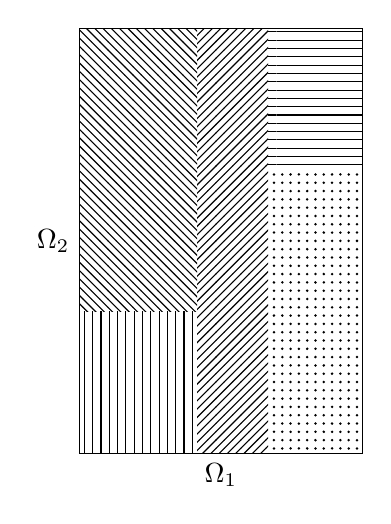
\begin{tikzpicture}[xscale=.6, yscale=.9]	
\fill [pattern=north west lines] (2.5,6) rectangle (0,2);
\fill [pattern=vertical lines] (2.5,2) rectangle (0,0);
\fill [pattern=north east lines] (2.5,0) rectangle (4,6);
\fill [pattern=horizontal lines] (4,4) rectangle (6,6);
\fill [pattern=dots] (4,0) rectangle (6, 4);
\draw [draw=black] (6,6) rectangle (0,0);
\node [below] at (3, 0) {$\Omega_1$};
\node [left] at (0, 3) {$\Omega_2$};
\end{tikzpicture}}
\caption{Illustration of sample space partitioning. (a) Partition of a two dimensional sample space $\Omega = \Omega_1 \times \Omega_2$ into $\{\mathcal P_1, \dots \mathcal P_5\}$ regions according to splitting points $\{s^*_0, \dots s^*_3\}$. Once the partition is obtained each each $\mathcal P_i$ predicts a constant output value (b).}
\label{sample_space_partition}
\end{figure}
 Recall, 
\begin{definition}[Partition]
	A partition $\mathcal P$ is a family of sets $\mathcal P = \{\mathcal P_i ~|~i\in I\}$ such that
	\begin{align*}
	\Omega = \bigcupdot_{i\in I} \mathcal P_i, ~ \mathcal P_i \neq \emptyset
	\end{align*}
\end{definition}
In practice, the partition is determined by a sequence of splitting points $(s^*_{\tau i_\tau})_{\tau = 0,\dots, k}$ \textit{in parallel} feature $i_\tau\in \{1,\dots, p\}$ in a \textit{non-commutative} way. Learning corresponds to finding the partition in sample space.


The partitioning process can be also understood as a (decision) tree structure. Start with a root node $\tau_0$ which corresponds to $\Omega$. Each node $\tau$ then splits sample space according to the splitting point $s^*_{\tau i}$  (Figure \ref{fig:decision_tree}). 
\begin{figure}
\centering
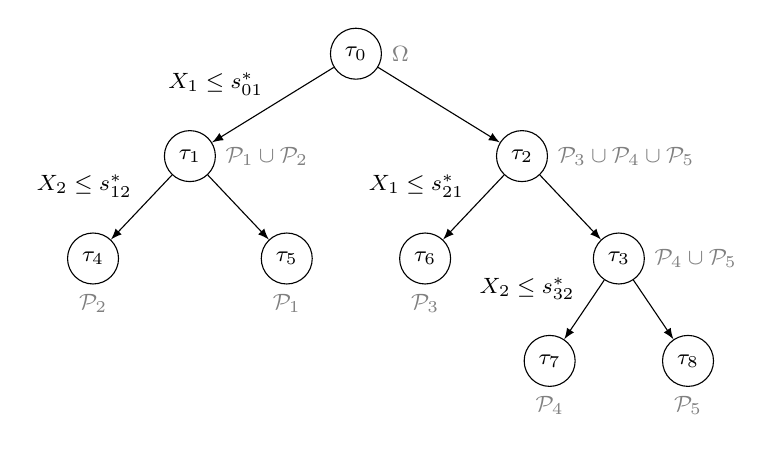
\begin{tikzpicture}[
grow                    = down,
sibling distance        = 12em,
level distance          = 3.7em,
edge from parent/.style = {draw, -latex},
every node/.style       = {font=\footnotesize},
level 2/.style={sibling distance=7em},
level 3/.style={sibling distance=5em},
treenode/.style = {circle, draw, align=center}
]

%\tikzstyle{every node}=[circle,draw]

\node [treenode, label=right:\textcolor{gray}{$\Omega$}] {$\tau_0$}
child {node [treenode, label=right:\textcolor{gray}{$\mathcal P_1 \cup \mathcal P_2$}] {$\tau_1$} 
	child {node [treenode, label=below:\textcolor{gray}{$\mathcal P_2$}] {$\tau_4$}
		   edge from parent node[above left, draw=none] {$X_2 \leq s_{12}^*$}}
	child {node [treenode, label=below:\textcolor{gray}{$\mathcal P_1$}] {$\tau_5$}}
           edge from parent node[above left, draw=none] {$X_1 \leq s_{01}^*$}}
child { node [treenode, label=right:\textcolor{gray}{$\mathcal P_3 \cup \mathcal P_4 \cup \mathcal P_5$}] {$\tau_2$}
	child {node [treenode, label=below:\textcolor{gray}{$\mathcal P_3$}] {$\tau_6$}
		   edge from parent node[above left, draw=none] {$X_1 \leq s_{21}^*$}}
	child {node [treenode, label=right:\textcolor{gray}{$\mathcal P_4 \cup \mathcal P_5$}] {$\tau_3$}
       child{node [treenode, label=below:\textcolor{gray}{$\mathcal P_4$}]{$\tau_7$}
             edge from parent node[above left, draw=none] {$X_2 \leq s_{32}^*$}}
       child{node [treenode, label=below:\textcolor{gray}{$\mathcal P_5$}]{$\tau_8$}}   
          }
      };
\end{tikzpicture}

\caption{Illustration of a binary decision tree for a single sample with features $(X_1, X_2)$. At each node the associated subspace of sample space is shown in gray. The sample is passed through the decision tree until it gets assigned to one of the leaf nodes $\{\tau_3, \tau_4, \tau_5, \tau_7, \tau_8\}$ that are associated with the sample space partition $\{\mathcal P_1, \dots \mathcal P_5\}$.}

\label{fig:decision_tree}
\end{figure}
 Note that this is a \textit{binary} decision tree, i.e., there are two child nodes at each split node. These are determined if the splitting criterion (e.g. $X_1 \leq s_{01}^*$ for the 0-th split) is fulfilled (left child node) or not (right child node). At the terminal (leaf) nodes there is no further split. The set of all terminal leaf nodes correspond to the partition of sample space. 
 
 We are aiming to build a tree where each node further partitions sample space. To this end, we consider nodes of the form $\tau=(\Omega_\tau, \mathcal S_\tau, \mathcal P_\tau)$. Where $\Omega_\tau \subset \Omega$ is a subspace, which is further partitioned by $\tau$ according to $\mathcal P_\tau$. We call $\Omega_\tau$ \textit{active  sample space} at node $\tau$. Furthermore we call the set $\mathcal S_{\tau} = \{(x, y) ~ | ~ (x, y) \in \mathcal S, ~  x \in \Omega_\tau\}$  \textit{active training set} at node $\tau$. Following the idea of sequentially partitioning sample space gives raise to 
 
 \begin{definition}[Decision tree]
 	A decision tree is a directed acyclic, singly connected graph with nodes $\{\tau ~ | ~\tau = (\Omega_\tau, \mathcal S_\tau, \mathcal P_\tau)\}$, where $\Omega_\tau$ is the active sample set, $\mathcal S_\tau$ is the active training set 
 	and $\mathcal P_\tau = \{\mathcal P_{\tau i} ~ | ~  i \in I_\tau\}$ 
 	is the partition of $\Omega_\tau$ such that: 
 	\begin{enumerate}
 		\item The root node is of the form  $\tau_0=(\Omega, \mathcal S, \mathcal P_{\tau_0})$
 		\item $\tau$ is leaf node $\Leftrightarrow |\mathcal P_\tau| = 1$   
 		\item $\tau$ has $|\mathcal P_\tau|$ child nodes for $|\mathcal P_\tau| >1$. Each child node $\tau_c$ has active sample set $\Omega_{\tau_c} = \mathcal P_{\tau c}, ~ c \in I_\tau$.
 	\end{enumerate} 
 \end{definition}
Apparently, this definition assures that for a decision tree the active sets of all leaf nodes $\{\Omega_\tau \mid \tau \text{ is leaf node}\}$ is indeed a partition of $\Omega$.

\paragraph{Examples}
\begin{itemize}
	 \item A binary decision tree is a decision tree where each non-terminal node has $|\mathcal P_\tau| = 2$. That is, each non-terminal node has exactly two child nodes.

	\item  Consider a node $\tau=(\Omega_\tau, \mathcal S_\tau)$ where all features in $S_\tau$ are ordered. Define a splitting point $s^*_{\tau i}$ along feature $i$. This induces a partition $\mathcal P_\tau = \{\mathcal P_l, \mathcal P_r\}$ with $\mathcal P_l = \{x ~|~ x\in\Omega_\tau,~ x_i \leq s^*_{\tau i}\}$ and $\mathcal P_r = \{x ~|~ x\in\Omega_\tau,~ x_i > s^*_{\tau i}\}$. Hence there are two child $\tau_l, \tau_r$   of node $\tau$ with active sample sets $\Omega_{\tau_l}=\mathcal P_l$ and $\Omega_{\tau_r}=\mathcal P_r$, respectively.
\end{itemize}
Within this point of view learning consists of 1) finding the decision tree structure (i.e., the node partitions $\mathcal P_\tau$) and 2) applying assignment rules at the leaf nodes.  
 

\subsection{Assigment rules on leaf nodes.}
Assume that we have learned in some way the decision tree and thus the partition of sample space (vie the leaf nodes). 
At the leaf nodes decision trees assign a constant value using the Bayes model. To this end we introduce a latent variable for the leaf node membership.
\begin{align}
	p(y, x, \tau) &= p(y \mid x, \tau)\, p(\tau, x) \\ 
	              &\approx p(y \mid \tau)\, p(\tau, x)  \label{approx:joint_pdf_dt}
\end{align}
where the approximation accounts for the basic idea that the prediction is only based on the partition $x$ falls into and not on its specific value. 
%and thus on the leaf node $x$ is member of. Thus the conditional probability, 
%\begin{align} \label{eq:cond_node_probability}
%p(\tau \mid x) = \mathbb 1(x \in \Omega_\tau, \tau \text{ is leaf %node})
%\end{align} 
Plugging this factorization into the expected loss function gives,
\begin{align}
	E_{XY\mathrm{T}} \left( L(Y, f(\mathrm{T})) \right) 
	&= \sum_{\tau}   \int_\Omega dx  \, p(\tau, x) \int dy\,L(y, f(\tau)) \, p(y \mid \tau)\,  \\
	&= \sum_{\tau}   p(\tau) \int dy\,L(y, f(\tau)) \, p(y \mid \tau')\,  
	%&= \int_{\Omega_\tau}   dx \, p(x) \int dy\,L(y, f(x)) p(y \mid \tau) 
	\label{eq:expected_loss_decision_tree},
\end{align}
where the model depends only on the node, $f(\tau)$, which is a consequence of factorization (\ref{approx:joint_pdf_dt}). Expression (\ref{eq:expected_loss_decision_tree}) is the expected loss over the whole model (i.e, including all nodes via the expectation value). By factorization (\ref{approx:joint_pdf_dt}) it does not depend on $x$.

Since we are interested in the assignment rule at a given leaf node,
we would like to compute the expected loss function conditioned on leaf node $\tau$, 
\begin{align}
E_{XY\mid\mathrm{T}} \left( L(Y, f(\mathrm{T})) \right) 
&=    \int_\Omega dx  \, p(x \mid  \tau ) \int dy\,L(y, f(\tau)) \, p(y \mid \tau)\,  \\
&=  \int dy\,L(y, f(\tau)) \, p(y \mid \tau')\,  
\label{eq:expected_cond_loss_decision_tree},
\end{align}
From (\ref{eq:expected_cond_loss_decision_tree}) or (\ref{eq:expected_loss_decision_tree}) and following the derivations for the Bayes model for classification (\ref{eq:bayes_classification}) and regression (\ref{eq:bayes_regression}) we therefore get as predictions at leaf node $\tau$:
\begin{itemize}\itemsep0em
	\item \textbf{Classification with zero-one loss}
	\begin{align} 
	\hat y_\tau &= \underset{y\in \Omega_t}{\operatorname{argmax}} ~ P(y\mid\tau) \label{eq:bayes_model_classification_dt}\\
	            &\approx
	            \underset{y\in \Omega_t}{\operatorname{argmax}}  \frac{N_{y\tau}}{N_\tau}  \label{approx:classification_tau}
	\end{align}
	where $N_{y\tau} = \lvert \{(x', y') \mid (x', y')  \in \mathcal S_\tau, ~ y'=y\}\rvert$ is the count of class labels in the active training set at node $\tau$ and
	$N_\tau =  \lvert \mathcal S_\tau \rvert$ is the size of the active training set.
	\item \textbf{Regression with squared loss}
	\begin{align}
	\hat y_\tau &= \int  y' p(y' \mid \tau)\, dy' \label{eq:bayes_model_regression_dt} \\ 
	 &\approx  \frac{1}{N_\tau} \sum_{i=1} ^{N_\tau}y_i.
	 \label{approx:regression_tau}
	\end{align}
\end{itemize}
So in classification problem, the class label is predicted by the maximum frequentist probability and in a regression problem the node value is given by the empirical mean.
The approximations refer to the frequentist estimates of the conditional probability (classification) and expectation value (regression) based on the active training sets at node $\tau$.

In summary, for a prediction at a leaf node we used approximation (\ref{approx:joint_pdf_dt}) and frequentist approximations (\ref{approx:classification_tau}) and (\ref{approx:regression_tau}). 
The first approximation neglects the specific value of $x$ and rather predicts globally on  the corresponding node. The second set of approximations has two implications \cite[Chapter~3.4]{understanding_random_forests}: 
First the frequentist approximation leads to unreliable estimates for nodes with small active training sets (in  particular, for nodes, which carry only one active training example). Second the estimates are based on the training data. Therefore we are taking the optimal decision not over the generalization error (as the Bayes model would do) but rather over the training set error.  This leads to the tendency of deep decision trees to severely overfit.


\subsection{Learning the tree structure.}
Among all possible decision trees for a learning task, training corresponds to finding that decision tree that minimizes the training set error. If there are several such candidates then Occam's Razor dictates to choose the smallest decision tree \cite{BLUMER1987377}, which is also simpler to interpret. However, finding the smallest tree that minimizes the training set error is an NP-complete problem \cite{HYAFIL197615}. Therefore, one needs to resort to heuristics. In essence, the tree is greedily/iteratively grown employing node splitting (partitioning) rules until a stopping criterion is met. To this end the following concepts are going to be introduced:
\begin{itemize}\itemsep0em 
	\item \textbf{Node partitioning rules} Instruction for finding the partitions $\mathcal P_\tau$ and a criterion for finding the "best" partition (goodness of split $\Delta i(\tau)$).
	\item \textbf{Greedy assumption:} grow the tree such that the goodness of split gets locally maximized.
	\item \textbf{Canonical stopping criteria:} This is used to determine whether a given node is split further or is a terminal (leaf) node. Consider a  node $\tau$ with active training set $\mathcal S_\tau$.  There are two cases that make $\tau$ a leaf node. First, if the target values of $\mathcal S_\tau$ are locally constant,
	\begin{align}
		y = y' ~  \forall (x,y), (x',y') \in  \mathcal S_\tau.
	\end{align}
	Second, if the features of $\mathcal S_\tau$ are locally constant,
	\begin{align}
	x = x' ~  \forall (x,y), (x',y') \in  \mathcal S_\tau.
	\end{align}
	As we are aiming to minimize the training set error, in the first case it does not make sense to further refine sample space, whereas in the second case sample space cannot be further partitioned.
	\item \textbf{Pre-pruning} aims prevent to grow too deep trees and thus overfitting. This approach introduces additional stopping criteria (maximum depth of terminal node, minimum number of training examples in a leaf node, threshold for the total decrease in impurity, minimum number of training example in each child node upon node split)
	\item \textbf{Post-pruning:} this is an alternative to pre-pruning. First the tree is fully developed and then nodes are sequentially removed that degrade the generalization error. While post-pruning typically works better for decision  trees, pruning in general is no longer required for tree based ensemble methods. 
\end{itemize}
This allows to formulate the general form of a binary decision tree algorithm as given in algorithm \ref{algo:decision-tree}.

\begin{algorithm} 
	\caption{Greedy induction of a binary decision tree with pre-pruning}\label{algo:decision-tree}
	\begin{algorithmic}[1]
		\Procedure{Build decision tree $(\mathcal S)$ }{} 
		\State Create a decision tree $f$ with root node $\tau_0$ 
		\State Create an empty stack $\mathcal N$ of \textit{open} nodes $(\tau, \mathcal S_\tau)$ 
		\State $\mathcal N$.PUSH($\tau_0, \mathcal S$)
		\While{$\mathcal N$ is not empty} 
		\State $\tau, \mathcal S_\tau = \mathcal N$.POP()
		\If {the stopping criterion is met for $\tau$}
		\State $\hat y_\tau = \text{some constant value}$ 
		\Else{}
		 \State Find split in $\mathcal S_\tau$: $$s^*= \underset{s\in Q}{\operatorname{argmax} \Delta i (s,\tau) }$$
		 \State Partition $\mathcal S_\tau = \mathcal S_{\tau_l} \cup \mathcal S_{\tau_r}$ according to $s^*$
		 \State Create child nodes $\tau_l, \tau_r$ of $\tau$
		 \State $\mathcal N$.PUSH($\tau_l, \mathcal S_{\tau_l}$)
		 \State $\mathcal N$.PUSH($\tau_r, \mathcal S_{\tau_r}$)
		\EndIf
		\EndWhile
		\Return $f$
		\EndProcedure
	\end{algorithmic}
\end{algorithm}

\subsection{Impurity measures for classification}
Intuitively a "good" split is a split that makes the child nodes purer. That is, the probability of a sample falling into a child node should be sharply peaked at one class label. Rather than working with the concept of purity, the complementary concept is used\cite{cart84}:

\begin{definition}[Impurity function] \label{def:impurity_function}An impurity function is a function $\phi: M \rightarrow \mathbb R$, where $M=\left\{p \mid p\in [0,1]^J, ~ \sum_{j=1}^J p_j=1\right\}$ such that
	\begin{itemize}\itemsep0em 
		\item $\phi$ is a maximum only the point $\left(\frac{1}{J}, \frac{1}{J}, \dots, \frac{1}{J}\right)$
		\item $\phi$ is a minimum at the point  $\left(1, 0, \dots, 0\right)$
		\item $\phi$ is symmetric
	\end{itemize}
\end{definition}
By symmetry also all permutations of $\left(1, 0, \dots, 0\right)$ are minimizers. This concept is applied to the decision tree
\begin{definition}[Node impurity measure] Given an impurity function and decision tree with node $\tau$, the impurity measure at node $\tau$ is defined as,
\begin{align*}
	i(\tau) = \phi(p(c_1\mid \tau), p(c_2\mid \tau), \dots, p(c_J\mid \tau)),
\end{align*}
where $p(c_1\mid \tau), ~ c_i \in \Omega_t$ are the conditional class probabilities.
\end{definition}
Having defined the impurity measure at a given node we would like to obtain a measure on how beneficial it is to add further child nodes (i.e., further partition sample space).
\begin{definition}[Goodness of split] \label{def:goodness_of_split}
	Let $\mathcal C_\tau=\left\{\tau' \mid \tau' \text{ is child of }\tau\right\}$. Then the goodness of split at node $\tau$ is defined as
	\begin{align*}
		\Delta i(\tau, \mathcal C_\tau) = i(\tau) - \sum_{\tau' \in \mathcal C_\tau} p(\tau' \mid \tau) i(\tau')
	\end{align*} 
\end{definition}
Note the difference between $p(\tau' \mid \tau)$ and $p(\tau' \mid \tau, x)$. While in the latter expression there is exactly one child node that has probability one (by construction of a decision tree), the former approach is less trivial and is typically approximated by the proportions of the active training sets of the child nodes with respect to the parent node.

So the basic idea of Definition \ref{def:goodness_of_split} is to take as measure the expected reduction of the node impurity measure upon adding further child nodes. Intuitively we would expect $\Delta i(\tau) \geq 0$. That is any addition of child nodes leads to a decrease in the goodness of split and in the worst case it does not  decrease the goodness of split. The class of impurity functions that fulfill this intuition may be characterized by \cite[Appendix of Chap. 4]{cart84}, \cite{Ripley1995}:
\begin{theorem} \label{thm:classification_impurity_functions}
	%Let there be any binary partition of node $\tau$ with child nodes $\{\tau_l, \tau_r\}$. 
	If the impurity function is strictly concave, then the goodness of split 
	\begin{align*}
	\Delta i(\tau, \mathcal C_\tau) \geq 0,
	\end{align*}
	with equality if, and only if, $p(c \mid \tau') =  p(c \mid \tau), ~ \forall \tau' \in \mathcal C_\tau$ and $\forall c \in \Omega_\tau$. 
\end{theorem}
\begin{proof}
	First show that $\sum_{\tau' \in \mathcal C_\tau} p(\tau' \mid \tau) p(c\mid\tau') =  p(c\mid\tau)$. Let $\tau'$ be a child node of $\tau$. Then, $p(\tau' \mid \tau) p(c\mid\tau') = \frac{p(\tau', \tau)}{p(\tau)}   p(c\mid\tau') = \frac{p(\tau \mid \tau') p(\tau')}{p(\tau)}   p(c\mid\tau') = p(c, \tau' \mid \tau)$, because $p(\tau \mid \tau') =1$ as $\tau'$ is child of $\tau$. Thus for the sum $\sum_{\tau' \in \mathcal C_\tau}  p(c, \tau' \mid \tau) =  p(c \mid \tau)$.  Apparently $p(\tau' \mid \tau) \geq 0$ and $\sum_{\tau' \in \mathcal C_\tau} (\tau' \mid \tau) = 1$. So we can use Jensens inequality to show the inequality statement:
	\begin{align*}\sum_{\tau' \in \mathcal C_t} p(\tau'\mid \tau) i(\tau') &= \sum_{\tau' \in \mathcal C_t} p(\tau'\mid \tau) \phi(p(c_1\mid \tau'),\dots, p(c_J\mid \tau')) \\
	& \leq \phi \left(\sum_{\tau' \in \mathcal C_t} p(\tau'\mid \tau)  p(c_1\mid\tau), \dots,  \sum_{\tau' \in \mathcal C_t} p(\tau'\mid \tau)  p(c_J\mid\tau)\right) \\
	& = \phi \left(p(c_1\mid\tau), \dots, p(c_J\mid\tau)\right)  \\
	& =  i(\tau).
	\end{align*}
	Now assume that $p(c \mid \tau') =  p(c \mid \tau), ~ \forall \tau' \in \mathcal C_\tau$ and $\forall c \in \Omega_\tau$. Then $\sum_{\tau' \in \mathcal C_t} p(\tau'\mid \tau) i(\tau') = i(\tau)\sum_{\tau' \in \mathcal C_t} p(\tau'\mid \tau) = i(\tau)$. Therefore $\Delta i(\tau, \mathcal C_\tau) = 0$. 
	
	\textbf{Todo:opposite direction}
\end{proof}

The most common strictly concave impurity functions encountered in practice are:
	\begin{align}
    i(\tau) &= - \sum_{c \in \Omega_t} p(c \mid t) \log_2 p(c \mid t) \quad \text{(Shannon Entropy)} \label{eq:shannon_impurity}, \\ 
    i(\tau) &= \sum_{c \in \Omega_t} p(c \mid \tau) (1 - p(c \mid \tau)) \quad \text{(Gini Index)} \label{eq:gini_impurity}.
    \end{align}
For practical calculations the empirical probabilities based on the training data are taken. Note that the goodness of split of the Shannon impurity is just the information gain. 

Comparing the Gini and Shannon impurity \cite{Breiman1996}, Gini prefers splits that put the largest class in one pure node while Shannon prefers to balance the size of the child nodes. For problems with small number of classes they should give similar results. However for many classes, Gini may produce trees that are too unbalanced high up in the tree, while the entropy lacks uniqueness. Note that there are many other impurity measures proposed in the literature \cite{gini_vs_twoing, epub1833,  BERZAL200331}. 

Empirically, as long as the impurity function is reasonable, it rather effects the structure of the decision tree (and thus the interpretation) rather than the accuracy.

\paragraph{Remark.}There is another strictly convex impurity function that suggests itself. Taking the conditional expected loss (\ref{eq:expected_cond_loss_decision_tree}) for a decision tree at node $\tau$ with the corresponding Bayes model for the zero-one loss (\ref{eq:bayes_model_classification_dt}), 
\begin{align} \label{eq:impurity_misclassification_rate}
	i(\tau) &= \sum_{c\in \Omega_t} \,L(c, \hat c_\tau) p(c \mid \tau)  \nonumber \\ 
	 &=\sum_{y\in \Omega_t} \, \mathbb 1 (c \neq \hat c_\tau) p(c \mid \tau)  \nonumber \\
	 &= 1 - p(\hat c_\tau \mid \tau)  \nonumber \\ 
	&= 1 - \underset{c\in \Omega_t}{\operatorname{max}} ~ p(c \mid\tau) \quad \text{(Misclassification error)}.
\end{align}    
The corresponding goodness of split is then the reduction of the misclassification  error upon adding child nodes. 
Despite the natural attractiveness of this impurity function it has two serious flaws: 1) it could lead to scenarios where all possible node splits have zero goodness of split and 2) it does not account for beneficial shifts in the probability distributions of the child nodes. 
The first point may happen when all child nodes have the same majority class \cite{cart84, understanding_random_forests} and thus, making this impurity function useless. The second point is problematic within the greedy tree growing algorithm. Thus, the misclassification error seems to short-sighted upon growing a tree \cite{cart84, hasties}.  On the other hand the misclassification rate is useful in post-pruning.

\subsection{Impurity measures for regression}
For the regression problem  impurity functions seem to be less well characterized in the literature. The reason is that the regression pendant of (\ref{eq:impurity_misclassification_rate})  is less problematic (in classification the main problems are rooted in the few number of classes). Computing the expected loss (\ref{eq:expected_cond_loss_decision_tree}) for a decision tree at node $\tau$ with the corresponding Bayes model for the squared loss gives the \textit{impurity function for a regression tree}:
(\ref{eq:bayes_model_regression_dt})
\begin{align} 
	i(\tau) & = \int dy\,L(y, f(x)) p(y \mid \tau) \nonumber \\
	 & =  \int dy\,(y -  \hat y_\tau)^2 \, p(y \mid \tau), \quad \hat y_\tau=\int  y' p(y' \mid \tau)\, dy'. \label{eq:impurity_measure_regression}
\end{align}
\paragraph{Remark.} There is an interesting relation between the expected loss (\ref{eq:impurity_measure_regression}) and the Gini index (\ref{eq:gini_impurity}) for binary classification tasks. Consider a two class problem, $c_1=0$ and $c_2=1$. The Gini index is given by $i_G(\tau) = 2\, p(c_1|\tau)\, p(c_2|\tau)$. On the other hand, if we were treating the classification problem as a regression, the expected loss (\ref{eq:impurity_measure_regression}) translates into $i_R(\tau) = \sum_i (c_i -\hat c)^2 p(c_i\mid \tau)$ with $\hat c = \sum_i c_i\,p(c_i \mid \tau) = p(c_2\mid \tau)$. Therefore, $i_R =  p(c_1|\tau)\, p(c_2|\tau)$. Therefore, 
$$i_R(\tau) = i_G(\tau) / 2.$$ So the Gini index for a two class problem is up to a factor of two equivalent to the expected loss in the regression problem.  In this sense the impurity function (\ref{eq:impurity_measure_regression}) is applicable to both, a regression problem and a binary classification problem. 

\subsection{Generating bianary node splits}
Once the impurity function is defined the optimal node splits may be found. Node splits are just partitions of the active sample space. While partitions are quite generic in practice often binary node splits are used. 

\paragraph{Categorical features}
For a categorical feature with $L$ levels $\left\{l_1, \dots, l_L\right\}$ there are in principle $2^{L-1} - 1$  partitions. For the  binary classification problem this may be reduced by
\begin{theorem}\label{thm:categorical_splits}
	Suppose a binary classification problem and given a stricly concave impurity function. For a categorical feature order the levels in increasing $p(c=1 \mid  l = l_i)$. Then a partition of the form $\left\{l_1, \dots, l_k\right\} \cup \left\{l_k+1, \dots, l_L\right\}$ maximises the goodness of split.
\end{theorem}
\begin{proof}
	A proof may be found in  Refs. \cite{Ripley1995, cart84}.
\end{proof}
Intuitively, all level leading to high probabilities of one class should be put together. 
Unfortunately theorem \ref{thm:categorical_splits} does not extend to multi class problems.
In practice exhaustive searches are applied for features with $L \leq 10$ and random sampling for features with more categories \cite{understanding_random_forests}.
\subsection{Decison Tree Algorithms}
Having all ingredients at hand we can summarize the specific decision tree algorithms. They mainly differ in the pruning strategies and the exact way to split nodes.
\begin{itemize}\itemsep0em 
	\item CART
	\item C4.5
	\item Patient rule induction method (PRIM)
	\item Multivariate adaptive regression splines (MARS)
	\item Hierarchical mixture of experts (HME)
	\item Combining neural networks and decision trees \cite{DBLP:journals/corr/abs-1711-09784}
	\item Bayesian approaches (Denison et al., 1998; Chipman et al., 1998, 2002, 2010)
\end{itemize}
Disadvantages: split only parallel to features.
\paragraph{Missing values}
Instead of the standard procedures with missing values (throwing away datapoints or fetures with missing values or imputing) decision trees offer additional possibilities:
\begin{itemize}
	\item "Missing" as a category. This is applicable to categorical predictors
	\item Surrogate variables.
	\item https://newonlinecourses.science.psu.edu/stat508/lesson/11
	\item https://people.cs.pitt.edu/~milos/courses/cs2750-Spring03/lectures/class19.pdf
	
\end{itemize}
\section{Ensemble methods}
\begin{itemize}\itemsep0em 
	\item Bagging
	\item Boosting
	\item Random Forest
	\item AdaBoos
	\item XGboost	
\end{itemize}
\section{Outlook}
\begin{itemize} \itemsep0em
	\item Additive models
	\item Support Vector machines
	\item Logistic regression
\end{itemize}
\section{Bias-Variance Decomposition}
\section{Model selection}
\section{Feature selection}

\bibliographystyle{plain}
\bibliography{paper}
\end{document}